\documentclass[12pt,]{article}
\usepackage{lmodern}
\usepackage{amssymb,amsmath}
\usepackage{ifxetex,ifluatex}
\usepackage{fixltx2e} % provides \textsubscript
\ifnum 0\ifxetex 1\fi\ifluatex 1\fi=0 % if pdftex
  \usepackage[T1]{fontenc}
  \usepackage[utf8]{inputenc}
\else % if luatex or xelatex
  \ifxetex
    \usepackage{mathspec}
  \else
    \usepackage{fontspec}
  \fi
  \defaultfontfeatures{Ligatures=TeX,Scale=MatchLowercase}
\fi
% use upquote if available, for straight quotes in verbatim environments
\IfFileExists{upquote.sty}{\usepackage{upquote}}{}
% use microtype if available
\IfFileExists{microtype.sty}{%
\usepackage{microtype}
\UseMicrotypeSet[protrusion]{basicmath} % disable protrusion for tt fonts
}{}
\usepackage[margin=1in]{geometry}
\usepackage{hyperref}
\PassOptionsToPackage{usenames,dvipsnames}{color} % color is loaded by hyperref
\hypersetup{unicode=true,
            pdftitle={Dashboards project},
            pdfauthor={Richard White},
            colorlinks=true,
            linkcolor=Maroon,
            citecolor=Blue,
            urlcolor=Blue,
            breaklinks=true}
\urlstyle{same}  % don't use monospace font for urls
\usepackage{natbib}
\bibliographystyle{apalike}
\usepackage{longtable,booktabs}
\usepackage{graphicx,grffile}
\makeatletter
\def\maxwidth{\ifdim\Gin@nat@width>\linewidth\linewidth\else\Gin@nat@width\fi}
\def\maxheight{\ifdim\Gin@nat@height>\textheight\textheight\else\Gin@nat@height\fi}
\makeatother
% Scale images if necessary, so that they will not overflow the page
% margins by default, and it is still possible to overwrite the defaults
% using explicit options in \includegraphics[width, height, ...]{}
\setkeys{Gin}{width=\maxwidth,height=\maxheight,keepaspectratio}
\IfFileExists{parskip.sty}{%
\usepackage{parskip}
}{% else
\setlength{\parindent}{0pt}
\setlength{\parskip}{6pt plus 2pt minus 1pt}
}
\setlength{\emergencystretch}{3em}  % prevent overfull lines
\providecommand{\tightlist}{%
  \setlength{\itemsep}{0pt}\setlength{\parskip}{0pt}}
\setcounter{secnumdepth}{5}
% Redefines (sub)paragraphs to behave more like sections
\ifx\paragraph\undefined\else
\let\oldparagraph\paragraph
\renewcommand{\paragraph}[1]{\oldparagraph{#1}\mbox{}}
\fi
\ifx\subparagraph\undefined\else
\let\oldsubparagraph\subparagraph
\renewcommand{\subparagraph}[1]{\oldsubparagraph{#1}\mbox{}}
\fi

%%% Use protect on footnotes to avoid problems with footnotes in titles
\let\rmarkdownfootnote\footnote%
\def\footnote{\protect\rmarkdownfootnote}

%%% Change title format to be more compact
\usepackage{titling}

% Create subtitle command for use in maketitle
\newcommand{\subtitle}[1]{
  \posttitle{
    \begin{center}\large#1\end{center}
    }
}

\setlength{\droptitle}{-2em}

  \title{Dashboards project}
    \pretitle{\vspace{\droptitle}\centering\huge}
  \posttitle{\par}
    \author{Richard White}
    \preauthor{\centering\large\emph}
  \postauthor{\par}
      \predate{\centering\large\emph}
  \postdate{\par}
    \date{2018-11-13}

\usepackage{booktabs}

\usepackage{amsthm}
\newtheorem{theorem}{Theorem}[section]
\newtheorem{lemma}{Lemma}[section]
\theoremstyle{definition}
\newtheorem{definition}{Definition}[section]
\newtheorem{corollary}{Corollary}[section]
\newtheorem{proposition}{Proposition}[section]
\theoremstyle{definition}
\newtheorem{example}{Example}[section]
\theoremstyle{definition}
\newtheorem{exercise}{Exercise}[section]
\theoremstyle{remark}
\newtheorem*{remark}{Remark}
\newtheorem*{solution}{Solution}
\begin{document}
\maketitle

{
\hypersetup{linkcolor=black}
\setcounter{tocdepth}{2}
\tableofcontents
}
\listoftables
\listoffigures
\section*{Preface}\label{preface}
\addcontentsline{toc}{section}{Preface}

The dashboards project is a project at FHI concerned with running
automated analyses on data. An automated analysis is any analysis that:

\begin{enumerate}
\def\labelenumi{\arabic{enumi}.}
\tightlist
\item
  Will be repeated multiple times in the future
\item
  Always has an input dataset with consistent file structure
\item
  Always has the same expected output (e.g.~tables, graphs, reports)
\end{enumerate}

\section{Introduction}\label{introduction}

\subsection{Executive summary}\label{executive-summary}

The dashboards project is a project at FHI concerned with running
automated analyses on data.

In principle, the dashboards project is split up into three parts:

\begin{enumerate}
\def\labelenumi{\arabic{enumi}.}
\tightlist
\item
  The umbrella infrastructure (i.e.~Docker containers, continuous
  integration, chron jobs, etc.)
\item
  The R package for each automated analysis
\item
  Integrating the R package into the physical system (e.g.~specifying
  where the data is)
\end{enumerate}

\subsection{What is an automated
analysis?}\label{what-is-an-automated-analysis}

An automated analysis is any analysis that:

\begin{enumerate}
\def\labelenumi{\arabic{enumi}.}
\tightlist
\item
  Will be repeated multiple times in the future
\item
  Always has an input dataset with consistent file structure
\item
  Always has the same expected output (e.g.~tables, graphs, reports)
\end{enumerate}

\subsection{Why not have one project for each automated
analysis?}\label{why-not-have-one-project-for-each-automated-analysis}

Automated analyses have a lot of code and infrastructure in common.

Automated analyses:

\begin{enumerate}
\def\labelenumi{\arabic{enumi}.}
\tightlist
\item
  Need their code to be tested via unit testing to ensure the results
  are correct
\item
  Need their code to be tested via integration testing to ensure
  everything runs
\item
  Need to be run at certain times
\item
  Need to be able to send emails notifying people that the analyses have
  finished running
\item
  Need to make their results accessible to the relevant people
\end{enumerate}

By combining them all in one umbrella project we can force everyone to
use the same infrastructure and coding principles, so we:

\begin{enumerate}
\def\labelenumi{\arabic{enumi}.}
\tightlist
\item
  Only need to solve a problem once
\item
  Only need to maintain one system
\item
  Can easily work on multiple projects, as we all speak the same
  language
\end{enumerate}

\subsection{Important repositories}\label{important-repositories}

\subsubsection{Infrastructure}\label{infrastructure}

\url{https://github.com/raubreywhite/dashboards_control/} (private)

This contains the Docker files, cronfiles, all bash scripts, etc.

\url{https://folkehelseinstituttet.github.io/dashboards/} (this one)

This contains the R executable for each automated analysis.

\url{https://folkehelseinstituttet.github.io/fhi/}

This is an R package that contains helper functions.

\subsubsection{Automated analyses R
packages}\label{automated-analyses-r-packages}

\url{https://folkehelseinstituttet.github.io/dashboards_sykdomspuls/}

\url{https://folkehelseinstituttet.github.io/dashboards_normomo/}

\url{https://folkehelseinstituttet.github.io/dashboards_sykdomspuls_pdf/}

\url{https://folkehelseinstituttet.github.io/dashboards_sykdomspuls_log/}

\section{Integrating the R package into the physical
system}\label{integrating-the-r-package-into-the-physical-system}

\subsection{Summary}\label{summary}

An R package is not enough to run an analysis -- something needs to
physically call the functions inside the R package. That is, the R
package needs to be integrated into the physical system.

Everything related to integrating the R package into the physical system
lives in the
\href{https://github.com/folkehelseinstituttet/dashboards/}{dashboards}
repository.

Inside the
\href{https://github.com/folkehelseinstituttet/dashboards/}{dashboards}
repository we have:

\begin{verbatim}
- dev/
  |-- src/
    |-- sykdomspuls/
       |-- 0_run.sh
       |-- RunProcess.R
       |-- RunTest.R
    |-- normomo/
       |-- 0_run.sh
       |-- RunProcess.R
       |-- RunTest.R
    |-- sykdomspuls_log/
       |-- 0_run.sh
       |-- RunProcess.R
       |-- RunTest.R
    |-- sykdomspuls_pdf/
       |-- 0_run.sh
       |-- RunProcess.R
       |-- RunTest.R
\end{verbatim}

\subsection{RunProcess.R}\label{runprocess.r}

\subsubsection{Aim}\label{aim}

An automated analysis needs to:

\begin{enumerate}
\def\labelenumi{\arabic{enumi}.}
\tightlist
\item
  Know the location of the data/results folders.
\item
  Check for new data in these folders. If no new data - then quit.
\item
  Load in the data.
\item
  Load in the analysis functions.
\item
  Run the analyses.
\item
  Save the results.
\end{enumerate}

\texttt{RunProcess.R} is responsible for these tasks.

We can think of it as an extremely short and extremely high-level script
that implements the analysis scripts.

Depending on the automated analysis \texttt{RunProcess.R} can be run
every two minutes (constantly checking for new data), or once a week
(when we know that data will only be available on a certain day/time).

\subsubsection{Bounded context}\label{bounded-context}

\begin{enumerate}
\def\labelenumi{\arabic{enumi}.}
\tightlist
\item
  Only one instance of \texttt{RunProcess.R} can be run at a time.
\item
  Data only exists on physical folders on the system.
\item
  The following folder structure exists on the system (here the name of
  the automated analysis is \texttt{ANALYSIS}):
\end{enumerate}

\begin{verbatim}
/data_raw/
  |-- ANALYSIS/
/data_clean/
  |-- ANALYSIS/
/data_app/
  |-- ANALYSIS/
/results/
  |-- ANALYSIS/
/src/
  |-- ANALYSIS/
     |-- 0_run.sh
     |-- RunProcess.R
     |-- RunTest.R
\end{verbatim}

Point \#1 is important because if \texttt{RunProcess.R} is run every 2
minutes (constantly checking for new data) but the analyses take 3 hours
to run, then we need to ensure that only one instance of
\texttt{RunProcess.R} can be run at a time.

Point \#2 is important because sometimes:

\begin{enumerate}
\def\labelenumi{\arabic{enumi}.}
\tightlist
\item
  Data files need to be downloaded from external SFTP servers
  (\href{https://folkehelseinstituttet.github.io/dashboards_normomo/}{normomo},
  \href{https://folkehelseinstituttet.github.io/dashboards_sykdomspuls_log/}{sykdomspulslog}).
\item
  Results files need to be uploaded to external SFTP servers
  (\href{https://folkehelseinstituttet.github.io/dashboards_sykdomspuls/}{sykdomspuls}).
\end{enumerate}

If we include code to download/upload the files from SFTP servers inside
\texttt{RunProcess.R} then it makes it very difficult to test
\texttt{RunProcess.R} (because we will then need to simulate SFTP
servers inside our testing infrastructure). If we know that
\texttt{RunProcess.R} only accesses files that are available on physical
folders in the system, then our testing infrastructure is a lot easier
to create and maintain.

\subsection{0\_run.sh}\label{run.sh}

\subsubsection{Aim}\label{aim-1}

The aim of \texttt{0\_run.sh} is to ensure that:

\begin{enumerate}
\def\labelenumi{\arabic{enumi}.}
\tightlist
\item
  Points 1 and 2 of the bounded context of \texttt{RunProcess.R} happen
\item
  Run \texttt{RunProcess.R}
\end{enumerate}

With regards to the bounded context, we ensure that only one instance of
\texttt{RunProcess.R} is run at a time through the use of
\texttt{flock}.

(If neccessary) with regards to the bounded context, we use
\texttt{sshpass}, \texttt{sftp}, and \texttt{ncftpput} to
download/upload files from SFTP servers.

We then run \texttt{RunProcess.R} with a standard call:

\begin{verbatim}
/usr/local/bin/Rscript /src/ANALYSIS/RunProcess.R
\end{verbatim}

\subsection{RunTest.R}\label{runtest.r}

\subsubsection{Aim}\label{aim-2}

The aim of \texttt{RunTest.R} is to perform integration testing on the
automated analysis. This integration testing is performed as part of the
Jenkins build pipeline.

\section{R packages}\label{r-packages}

\subsection{Summary}\label{summary-1}

Each automated analysis has its own R package:

\begin{itemize}
\tightlist
\item
  \href{https://folkehelseinstituttet.github.io/dashboards_sykdomspuls/}{sykdomspuls}
\item
  \href{https://folkehelseinstituttet.github.io/dashboards_normomo/}{normomo}
\item
  \href{https://folkehelseinstituttet.github.io/dashboards_sykdomspuls_pdf/}{sykdomspulspdf}
\item
  \href{https://folkehelseinstituttet.github.io/dashboards_sykdomspuls_log/}{sykdomspulslog}
\end{itemize}

Each R package contains all of the code necessary for that automated
analysis. Typical examples are:

\begin{itemize}
\tightlist
\item
  Data cleaning
\item
  Signal analysis
\item
  Graph generation
\item
  Report generation
\end{itemize}

\subsection{Requirements}\label{requirements}

The R packages should be developed using unit testing as implemented in
the \href{http://r-pkgs.had.co.nz/tests.html}{testthat} package.

Furthermore, the R package should operate (and be able to be tested)
independently from the real datasets on the system. This is because the
real datasets cannot be shared publically or uploaded to github. To
circumvent this issue, each package will need to develop functions that
can generate fake data.
\href{https://folkehelseinstituttet.github.io/dashboards_sykdomspuls/reference/GenFakeDataRaw.html}{GenFakeDataRaw}
is one example from
\href{https://folkehelseinstituttet.github.io/dashboards_sykdomspuls/}{sykdomspuls}.

We also require that unit tests are created to test the
formatting/structure of results.
\href{https://folkehelseinstituttet.github.io/dashboards_sykdomspuls/reference/ValidateAnalysisResults.html}{ValidateAnalysisResults}
is one example from
\href{https://folkehelseinstituttet.github.io/dashboards_sykdomspuls/}{sykdomspuls},
where the names of the data.table are checked against reference values
to ensure that the structure of the results are not accidentally
changed.

\subsection{Deployment via travis-ci and
drat}\label{deployment-via-travis-ci-and-drat}

Unit testing is then automatically run using
\href{http://r-pkgs.had.co.nz/check.html\#travis}{travis-ci}. If the R
package passes all tests, then we use
\href{https://github.com/eddelbuettel/drat}{drat} to deploy a built
version of the package to Folkehelseinstituttet's R repository:
\url{https://folkehelseinstituttet.github.io/drat/}.

\section{Umbrella Infrastructure}\label{umbrella-infrastructure}

\begin{itemize}
\tightlist
\item
  Three computers
\end{itemize}

\subsection{Executive summary}\label{executive-summary-1}

The dashboards project is a project at FHI concerned with running
automated analyses on data.

In principle, the dashboards project is split up into three parts:

\begin{enumerate}
\def\labelenumi{\arabic{enumi}.}
\tightlist
\item
  The overarching infrastructure (i.e.~Docker containers, continuous
  integration, chron jobs, etc.)
\item
  The R package for each automated analysis
\item
  The executable for each automated analysis
\end{enumerate}

\subsection{What is an automated
analysis?}\label{what-is-an-automated-analysis-1}

An automated analysis is any analysis that:

\begin{enumerate}
\def\labelenumi{\arabic{enumi}.}
\tightlist
\item
  Will be repeated multiple times in the future
\item
  Always has an input dataset with consistent file structure
\item
  Always has the same expected output (e.g.~tables, graphs, reports)
\end{enumerate}

\subsection{Why not have one project for each automated
analysis?}\label{why-not-have-one-project-for-each-automated-analysis-1}

Automated analyses have a lot of code and infrastructure in common.

Automated analyses:

\begin{enumerate}
\def\labelenumi{\arabic{enumi}.}
\tightlist
\item
  Need their code to be tested via unit testing to ensure the results
  are correct
\item
  Need their code to be tested via integration testing to ensure
  everything runs
\item
  Need to be run at certain times
\item
  Need to be able to send emails notifying people that the analyses have
  finished running
\item
  Need to make their results accessible to the relevant people
\end{enumerate}

By combining them all in one umbrella project we can force everyone to
use the same infrastructure, so we:

\begin{enumerate}
\def\labelenumi{\arabic{enumi}.}
\tightlist
\item
  Only need to solve a problem once
\item
  Only need to maintain one system
\item
  Can easily work on multiple projects, as we all speak the same
  language
\end{enumerate}

\section{Contributing}\label{contributing}

\subsection{Development guidelines}\label{development-guidelines}

We try to follow the
\href{https://guides.github.com/introduction/flow/}{GitHub flow} for
development.

\begin{enumerate}
\def\labelenumi{\arabic{enumi}.}
\item
  Fork {[}this repo{]}{[}repo{]} and clone it to your computer. To learn
  more about this process, see
  \href{https://guides.github.com/activities/forking/}{this guide}.
\item
  Add the Folkehelseinstituttet repository as your upstream:

\begin{verbatim}
git remote add upstream https://github.com/folkehelseinstituttet/ORIGINAL_REPOSITORY.git
\end{verbatim}
\item
  If you have forked and cloned the project before and it has been a
  while since you worked on it, merge changes from the original repo to
  your clone by using:

\begin{verbatim}
git fetch upstream
git merge upstream/master
\end{verbatim}
\item
  Open the RStudio project file (\texttt{.Rproj}).
\item
  Make your changes:

  \begin{itemize}
  \tightlist
  \item
    Write your code.
  \item
    Test your code (bonus points for adding unit tests).
  \item
    Document your code (see function documentation above).
  \item
    Do an \texttt{R\ CMD\ check} using \texttt{devtools::check()} and
    aim for 0 errors and warnings.
  \item
    Commit your changes locally
  \item
    Merge changes from the original repo (again)
  \item
    Do an \texttt{R\ CMD\ check} using \texttt{devtools::check()} and
    aim for 0 errors and warnings.
  \end{itemize}
\item
  Commit and push your changes.
\item
  Submit a
  \href{https://guides.github.com/activities/forking/\#making-a-pull-request}{pull
  request}.
\item
  If you are reviewing the pull request, wait until the
  \href{www.travis-ci.org}{travis-ci} unit tests have finished
\end{enumerate}

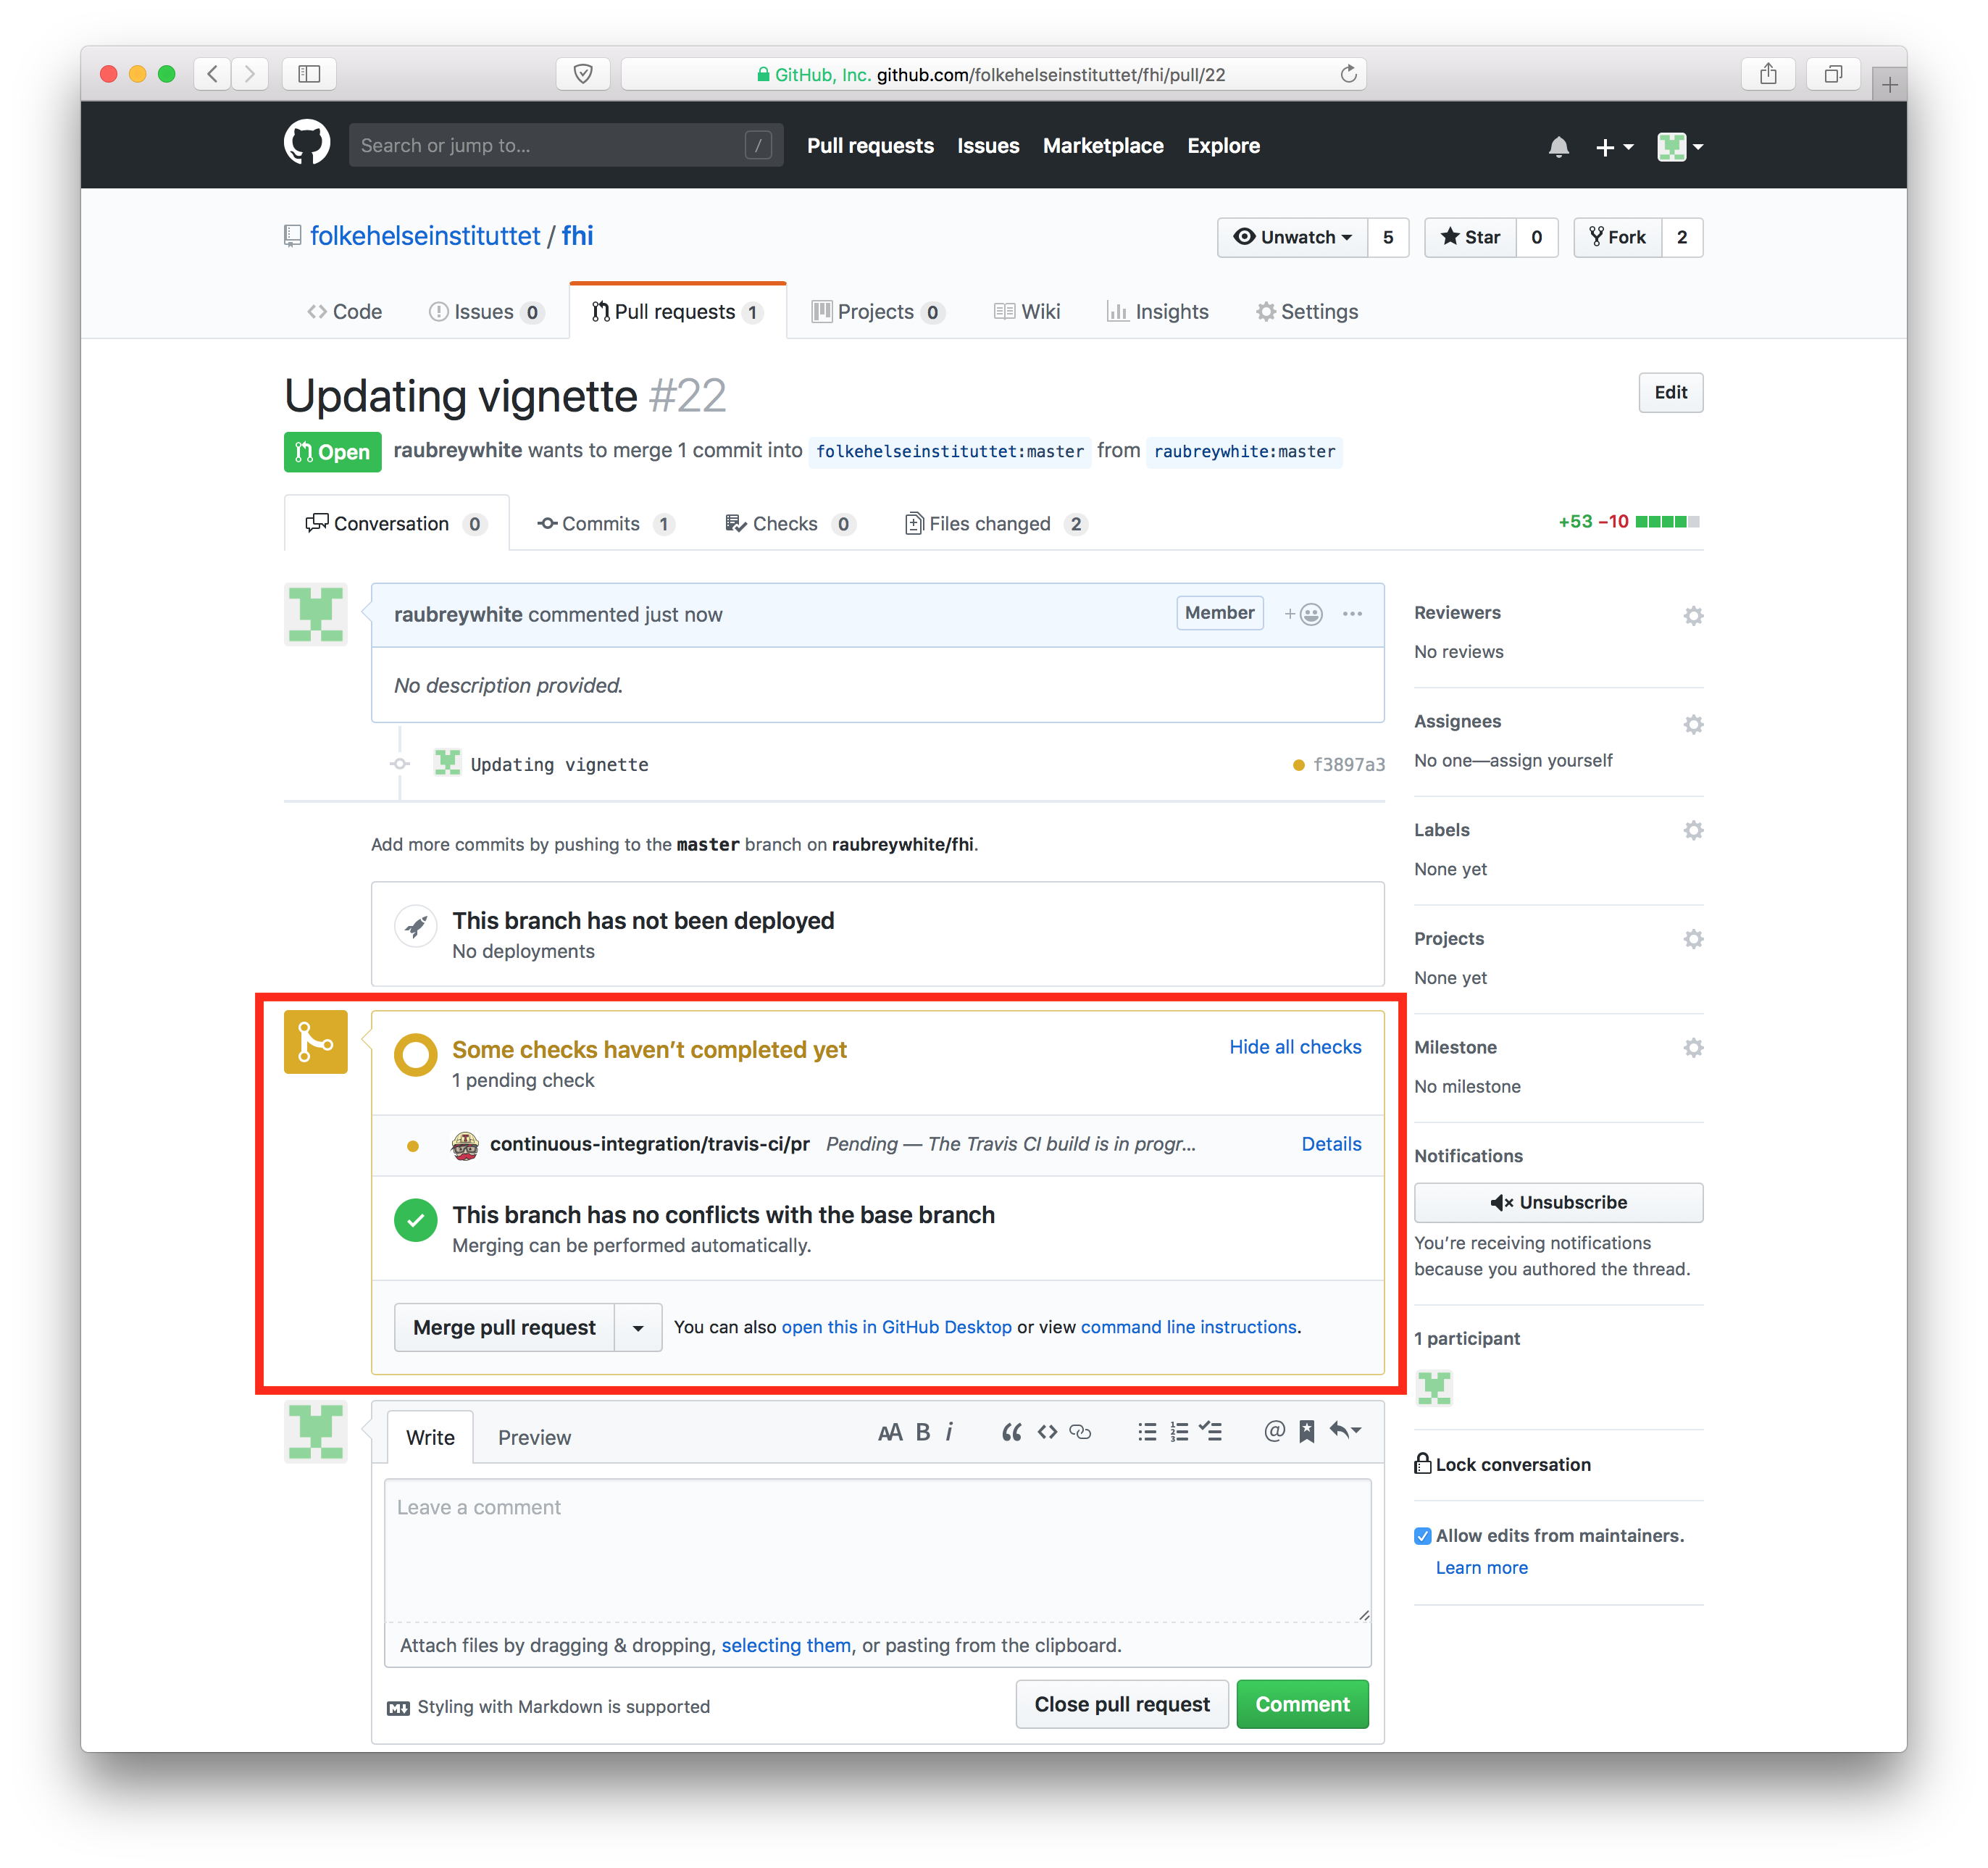
\includegraphics[width=38.11in]{images/pull_request_before_checks}

\begin{enumerate}
\def\labelenumi{\arabic{enumi}.}
\setcounter{enumi}{8}
\tightlist
\item
  Please make sure that the unit tests \texttt{PASS} before merging in!!
\end{enumerate}

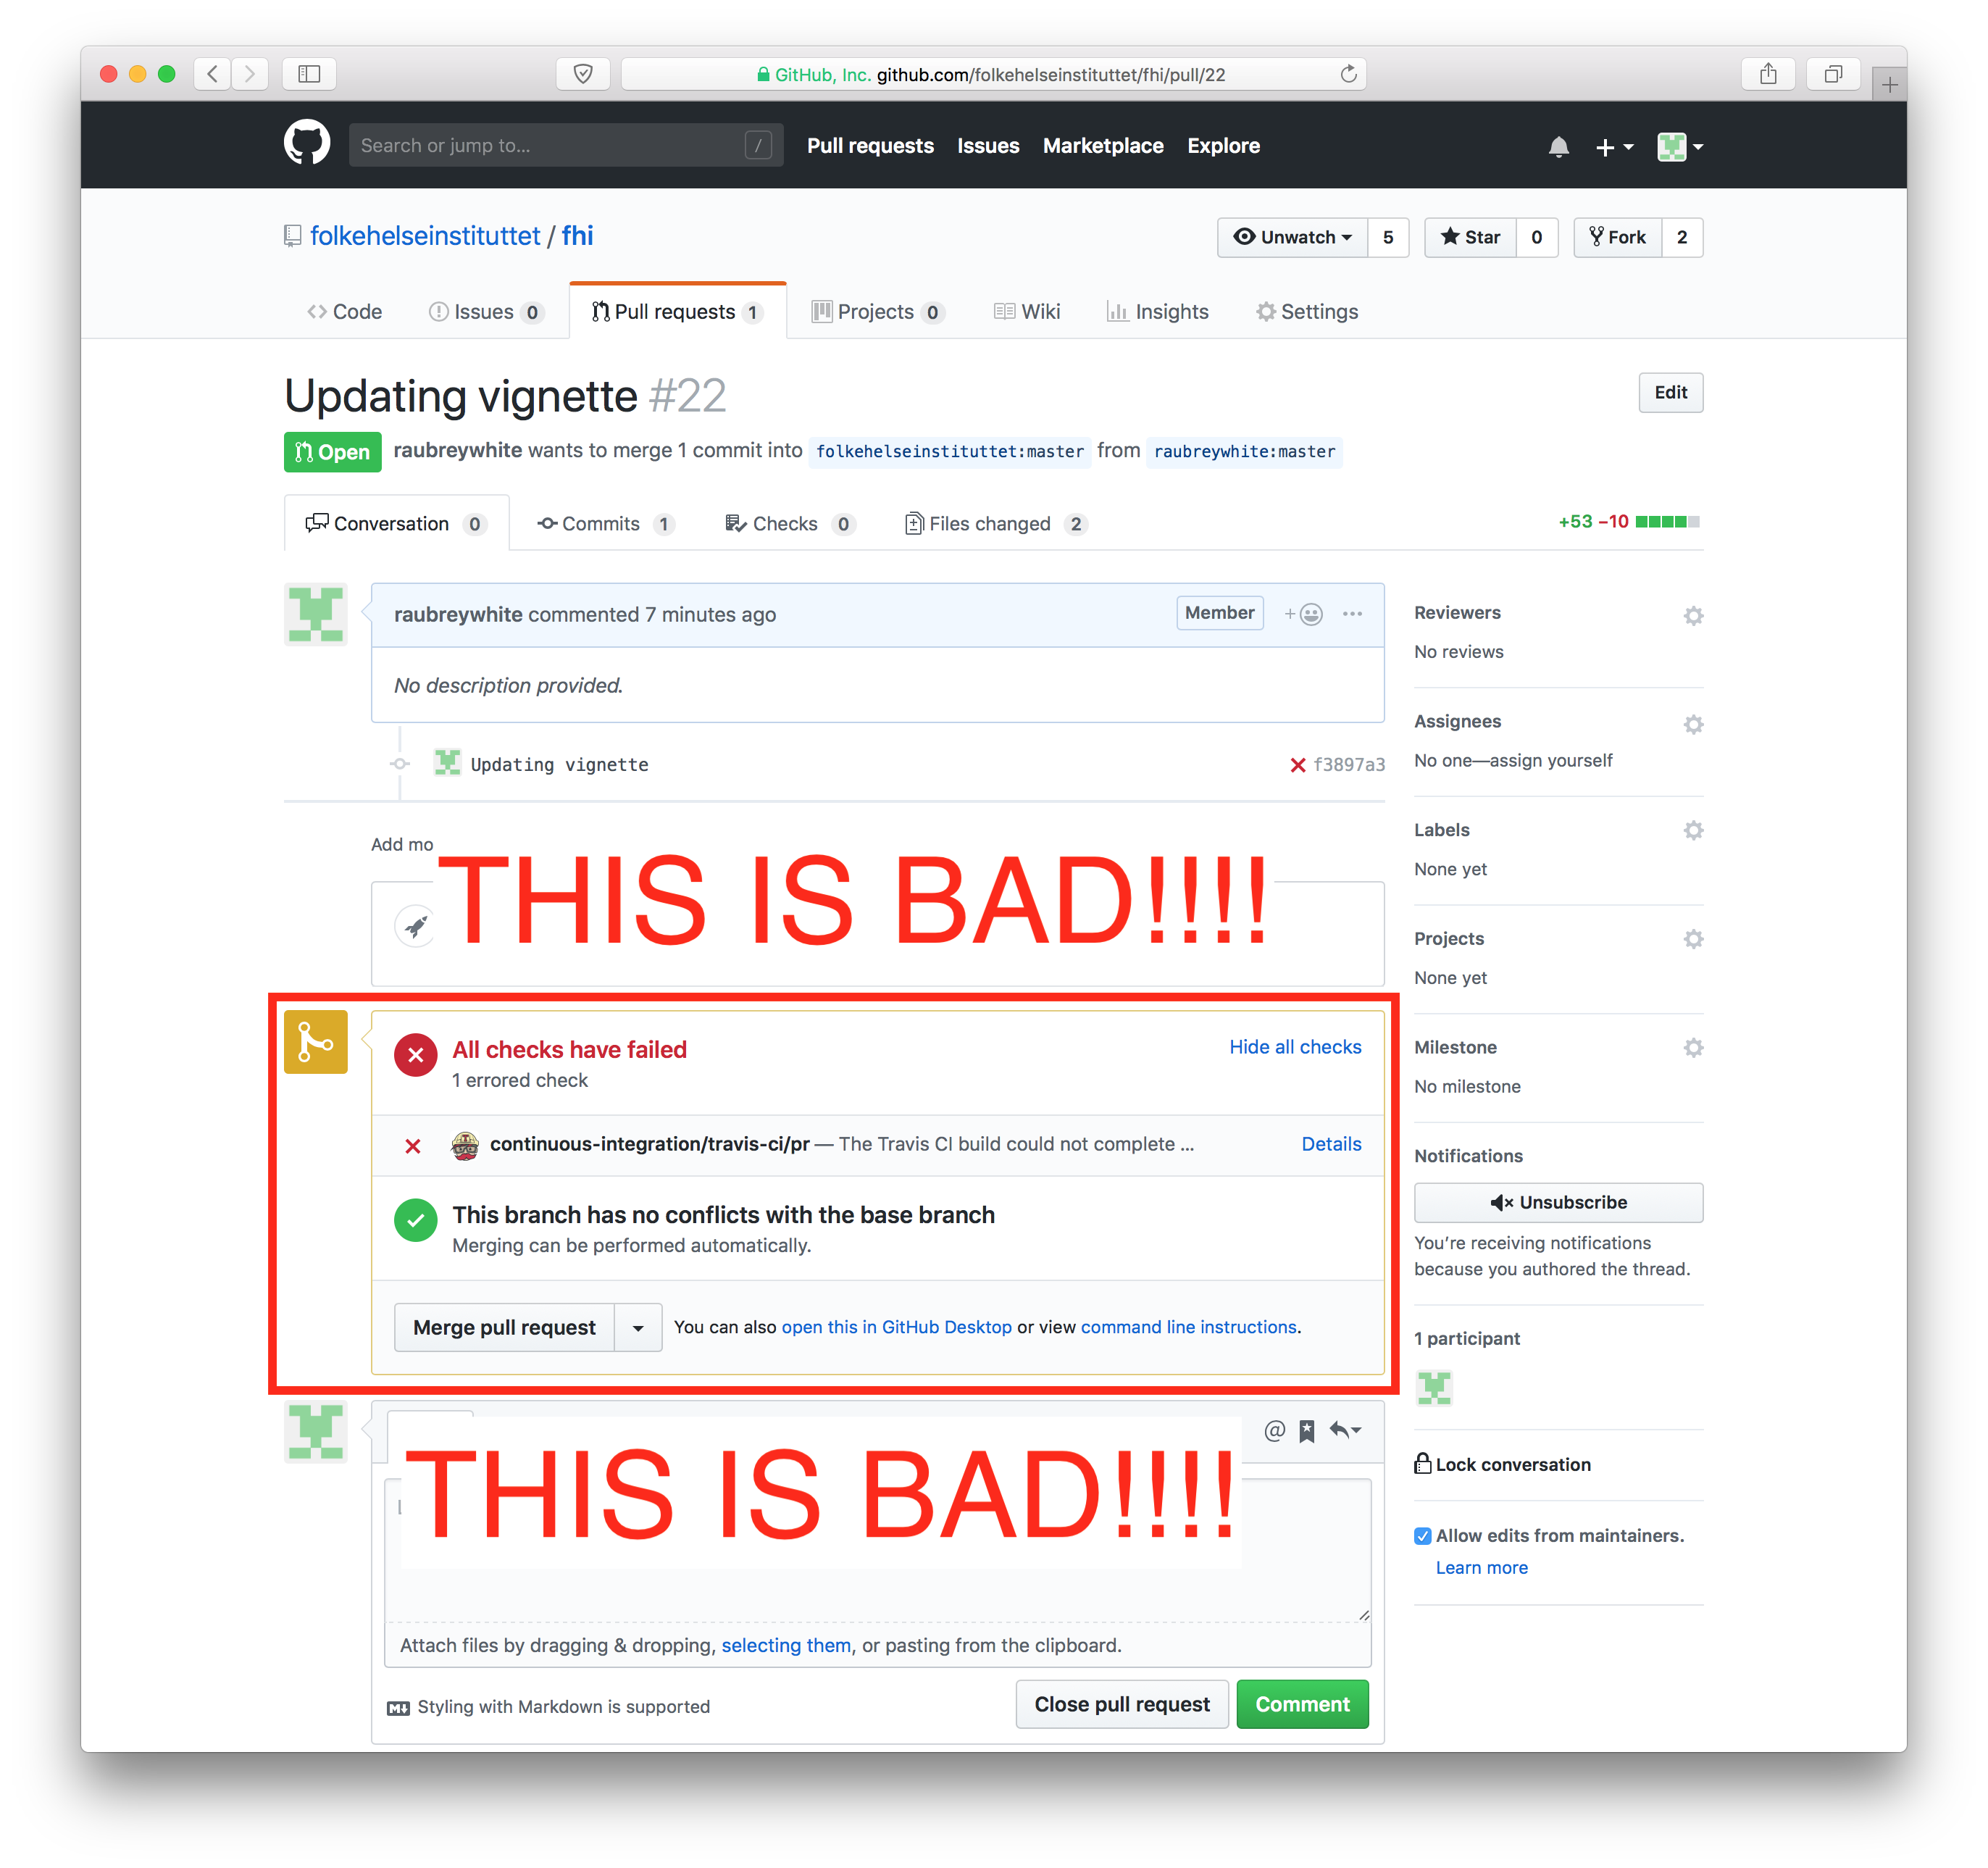
\includegraphics[width=38.11in]{images/pull_request_checks_failed}

\subsection{Code style}\label{code-style}

\begin{itemize}
\item
  Function names start with capital letters
\item
  Variable names start with small letters
\item
  Environments should be in ALL CAPS
\item
  Reference \href{http://adv-r.had.co.nz/Style.html}{Hadley's style
  code}
\item
  \textless{}- is preferred over = for assignment
\item
  Indentation is with two spaces, not two or a tab. There should be no
  tabs in code files.
\item
  if () \{\} else \{\} constructions should always use full curly braces
  even when usage seems unnecessary from a clarity perspective.
\item
  TODO statements should be opened as GitHub issues with links to
  specific code files and code lines, rather than written inline.
\item
  Follow Hadley's suggestion for aligning long functions with many
  arguments:

\begin{verbatim}
 long_function_name <- function(a = "a long argument", 
                            b = "another argument",
                            c = "another long argument") {
   # As usual code is indented by two spaces.
 }
\end{verbatim}
\item
  Never use print() to send text to the console. Instead use message(),
  warning(), and error() as appropriate.
\item
  Use environment variables, not options(), to store global arguments
  that are used by many or all functions.
\end{itemize}

\section{Manual Actions}\label{manual-actions}

\subsection{Sykdomspulsen}\label{sykdomspulsen}

\subsubsection{Sykdomspulsen Weekly
update}\label{sykdomspulsen-weekly-update}

The weekly update needs to be done every Tuesday morning. New data has
arrived from Helsedirektoratet to FHI during Monday evening and night,
and the further statistical analysis and updating of the interactive
webpage for Sykdomspulsen is done on Tuesday. For more information about
Sykdomspulsen setup:

\url{https://folkehelseinstituttet.github.io/dashboards/}

\url{https://folkehelseinstituttet.github.io/dashboards_sykdomspuls/}

\begin{enumerate}
\def\labelenumi{\arabic{enumi}.}
\tightlist
\item
  Log in to «Sikker sone»
\item
  Click on «Sikkersone statistikk»
\item
  Open R or R studio by clicking on the four squares in the bottom left
  corner, then on the arrow pointing downwards approximately in the same
  area and search for R in the upper right corner
\item
  When R is open, click on ``file'' in the upper left corner, and then
  ``open script''
\item
  Open
  G:/Helseregistre/MSIS/Sykdomspulsen/Gry/FormattingWithinSikkersone/\\
  SykdomspulsenWeeklyReport
\item
  Slide the R-code so that it is beside the R console (so that you can
  see the whole R console)
\item
  Put the marker within the R-code and click Ctrl+A, then click Ctrl+R
\item
  After a few minutes, you will see a progress bar on the R-console,
  which shows how much of the code is finished. When the bar shows
  100\%, the whole code has run, and the results are finished (this
  takes about 1 hour, you can do other things while waiting for this)
\item
  When the progress bar shows 100\% you should look at the data that is
  shown in the console and see if the dates are from this week. If not
  you should contact the IT department by Cathrine Slorbak
  (\href{mailto:Cathrine.Slorbak@fhi.no}{\nolinkurl{Cathrine.Slorbak@fhi.no}})
  and Gry Grøneng
  (\href{mailto:GryMarysol.Groneng@fhi.no}{\nolinkurl{GryMarysol.Groneng@fhi.no}}).
  There is probably something wrong with receiving the data from the
  Health directorate, hence the IT department needs to solve it. Do not
  continue until the problem is solved.
\item
  If the dates look ok, you can close R (by clicking on x in the upper
  right corner).
\item
  Go to ``Windows explorer'' by clicking on the four squares in the
  lower left corner (still in ``sikker sone''), and go to:
  G:/Helseregistre/MSIS/Sykdomspulsen/Gry/\\
  FormattingWithinSikkersone, and find a text file which is called
  ``partially\_formatted\_\\
  todays date.txt'' (todays date is displayed 2017\_06\_13). You should
  look if the file is larger than last weeks file, it should be larger
  since we take out all the data every week, and more days have been
  added since last week. If the file is smaller than last week, contact
  the IT department by Cathrine Slorbak
  (\href{mailto:Cathrine.Slorbak@fhi.no}{\nolinkurl{Cathrine.Slorbak@fhi.no}})
  and Gry Grøneng
  (\href{mailto:GryMarysol.Groneng@fhi.no}{\nolinkurl{GryMarysol.Groneng@fhi.no}}).
  Do not continue until the problem is solved.
\item
  Copy and paste the file into the folder ``Filer til ordinær sone
  (J:)''
\item
  Log out of ``sikker sone'' and open the windows explorer in the
  ordinary zone and go to ``Filer overført fra sikker sone (K:)'' and
  find the file.
\item
  Copy and paste the file into:
\end{enumerate}

\begin{itemize}
\tightlist
\item
  F:/Prosjekter/sMSIS/WeeklyUpdates\_Sykdomspulsen AND
\item
  F:/Prosjekter/Dashboards/data\_raw/sykdomspuls
\end{itemize}

\begin{enumerate}
\def\labelenumi{\arabic{enumi}.}
\setcounter{enumi}{14}
\tightlist
\item
  You have now done the weekly update of Sykdomspulsen!
\end{enumerate}

\bibliography{book.bib}


\end{document}
